\documentclass{article}

\usepackage{shyne}

% document format
\topmargin 0in
\oddsidemargin 0in
\evensidemargin 0in
\headheight 0in
\headsep 0in
\topskip 0in
\textheight 9in
\textwidth 6.5in
\linespread{1.3}

\begin{document}

\begin{flushleft}
\section*{Group Work - Chapter 6}
\paragraph{1}
\begin{enumalpha}
\item The time it takes to finish a statistics midterm in a certain class is uniformly distributed between 1 and 2 hours (60 to 120 minutes). What is the probability that a randomly selected student will finish the exam in less than 75 minutes? What is the probability they will complete it between 100 and 110 minutes?\\
\medskip
{\centering
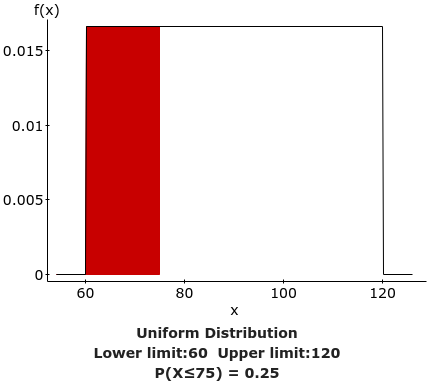
\includegraphics[width=2.5in]{images/grp06_Q1_a_1} \qquad
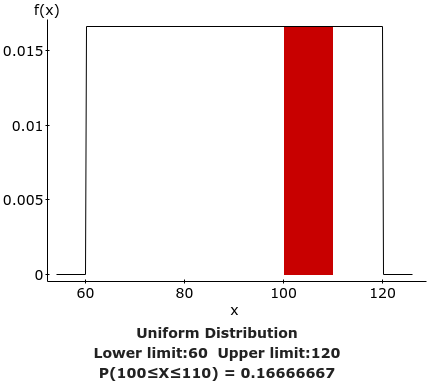
\includegraphics[width=2.5in]{images/grp06_Q1_a_2}
\par}
$\ds\bv{P(X < 75) = \frac {75 - 60}{120-60} = \frac{15}{60} = \frac 1 4 = 0.25}$\\
\medskip
$\ds\bv{P(100 < X < 110) = \frac{110 - 100}{120 -60} = \frac {10}{60} = \frac 1 6 = 0.167}$
\vspace{.5in}

\item The scores of the midterm are normally distributed and reported as z-scores. What is the probability of a random student getting a grade greater than $z = -0.5$? What is the grade ($z$-score) that separates the bottom 90\% of the class from the top 10\%?\\
\medskip
{\centering
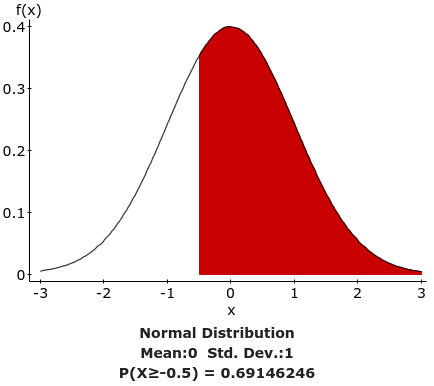
\includegraphics[width=2.5in]{images/grp06_Q1_b_1} \qquad
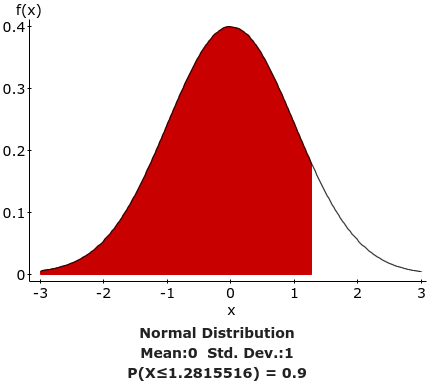
\includegraphics[width=2.5in]{images/grp06_Q1_b_2}
\par}
$\ds\bv{P(Z > -0.5) = 0.691}$\\
\medskip
$\ds\bv{P(Z < z) = 0.9, \qquad z = 1.28}$
\end{enumalpha}



\newpage
\paragraph{2} A new breakfast cereal ``Super Fruity Taco Bombs" is packaged by a machine which puts the cereal in the bag. The amount loaded by the machine is normally distributed with a mean of 14.5 ounces with a standard deviation of 1.15 ounces. A bag is rejected if it weighs less than 13 ounces.
\begin{enumalpha}
\item What is the proportion of bags of cereal that are rejected? What is the probability that a bag weighs between 15 and 16 ounces?\\
\medskip
{\centering
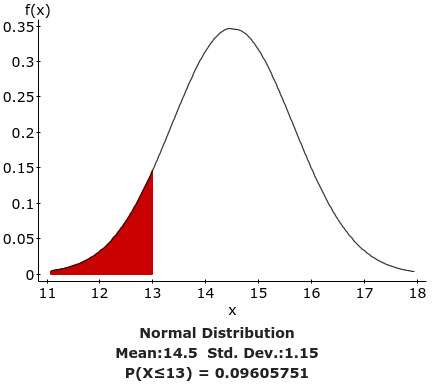
\includegraphics[width=2.5in]{images/grp06_Q2_a_1} \qquad
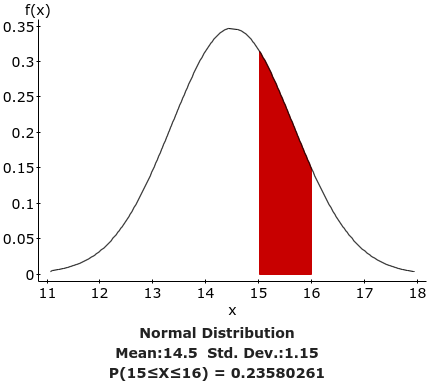
\includegraphics[width=2.5in]{images/grp06_Q2_a_2}
\par}
$\ds\bv{P(X < 13) = 0.096}$\\
\medskip
$\ds\bv{P(15 < X < 16) = 0.235}$
\vspace{.5in}

\item The company doesn't want to check each bag individually, so it begins weighing cases of 16 bags of cereal, rejecting a case if the mean weight of the bags is less than 13 ounces. Can we apply the CLT to this procedure? What proportion of cases get rejected? Is this procedure fair to the consumer?\\
\medskip
\bt{We can use the Central Limit Theorem because the population of bag weights is normally distributed.}\\
\medskip
$\ds\bv{\mu_{\bar x} = \mu = 14.5, \qquad \sigma_{\bar x} = \frac{\sigma}{\sqrt n} = \frac {1.15}{\sqrt{16}} = \frac {1.15}4 = 0.2875}$\\
\smallskip
{\centering
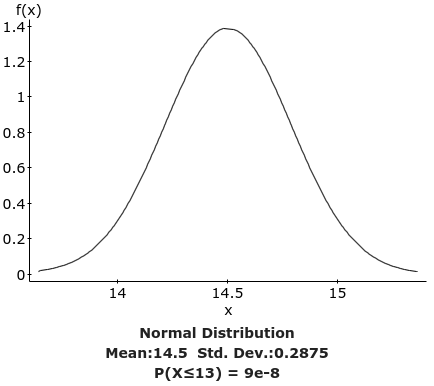
\includegraphics[width=2.5in]{images/grp06_Q2_b}
\par}
$\ds\bv{P(\bar x < 13) = 0.9 \times 10^{-8}}$\\
\medskip
\bt{This method would not be fair because it is possible to get a case which is accepted with one or more boxes that are under weight.}

\end{enumalpha}

\newpage
\newpage
\paragraph{3} Researchers are interested in understanding the factors affecting sleep quantity. A large longitudinal study found sleep per night was normally distributed with a mean of 420 minutes (8 hours) and a standard deviation of 80 minutes. Extreme sleep is defined as less than 6 hours (360 minutes) or more that 8 hours (420 minutes).
\begin{enumalpha}
\item What is the probability of a randomly selected subject having an extremely low amount of sleep per night? What is the probability of a subject having an extremely high amount of sleep?\\
\medskip
{\centering
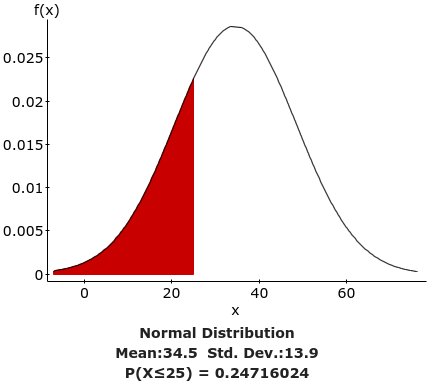
\includegraphics[width=2.5in]{images/grp06_Q3_a_1} \qquad
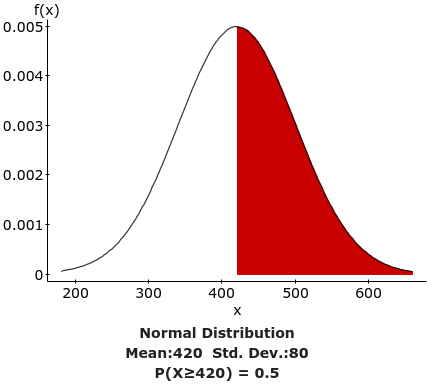
\includegraphics[width=2.5in]{images/grp06_Q3_a_2}
\par}
$\ds\bv{P(X < 360) = 0.227}$\\
\medskip
$\ds\bv{P(X > 420) = 0.5}$
\vspace{.4in}
\item The researchers would like to gather more detailed data on a sample from the larger study. If they select samples of 25 subjects, what is the probability that the sample has, on average, extremely low sleep? What is the probability the sample has extremely high sleep?\\
\medskip
\bt{We can use the Central Limit Theorem because the population of ages is normally distributed.}\\
\medskip
$\ds\bv{\mu_{\bar x} = \mu = 420	, \qquad \sigma_{\bar x} = \frac{\sigma}{\sqrt n} = \frac {80}{\sqrt{25}} = \frac {80}5 = 16}$\\
\medskip
{\centering
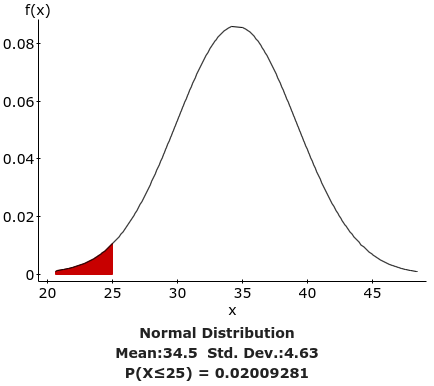
\includegraphics[width=2.5in]{images/grp06_Q3_b_1} \qquad
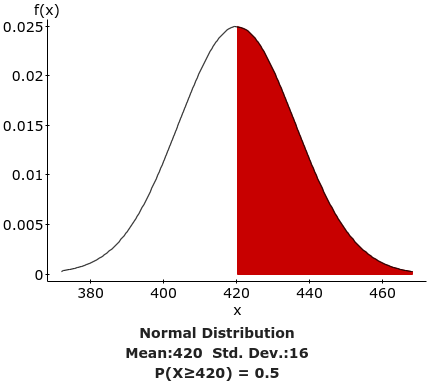
\includegraphics[width=2.5in]{images/grp06_Q3_b_2}
\par}
$\ds\bv{P(\bar x < 360) = 8.84 \times 10^{-5}}$\\
\medskip
$\ds\bv{P(\bar x > 60) = 0.5}$

\end{enumalpha}


\end{flushleft}
\end{document}